% !TEX root = ../my-thesis.tex
%
\chapter{Code Design}
\label{sec:code:model}

Machine learning (ML) models are algorithms that use data and statistical operations to optimize the weights that compose the model.
There are two broad catagories of ML models, supervised and unsupervised.
Supervised models are ones which use labeled data, or data which the expected output of the model is known in advance.
Unsupervised models are models for which a pattern is learned from the data directly.
The model use for this project is a supervised ML model because we know what the expected inputs and outputs should be and can produce labels for both.

The primary input for the model will be thermal images taken from the internal cameras at W7X.
Since the thermal camera data is sparse, with most of the pixels for any given shot containing zeros or noise, a convolutional neural network with that is optimized for sparse data would be ideal.



Convolutional neural networks use two dimensional convolutions applied to the inputs to generate new features (see Fig. \ref{fig:code:2DConv}).
These convolutions are stacked, being applied to the same input to produce multiple outputs which are concatenated along the z-axis.
Typically, strides (the number of pixels skipped over when translating the kernel) and padding (adding pixels around the edge of the image) allow convolutions to change the output x and y dimensions.
So as more layers of convolutions are successively applied, the outputs of each layer grow in z-height, and shrink in x and y.
The final output of the convolutional network is then passed to a fully connected network.


\begin{figure}[htb]
    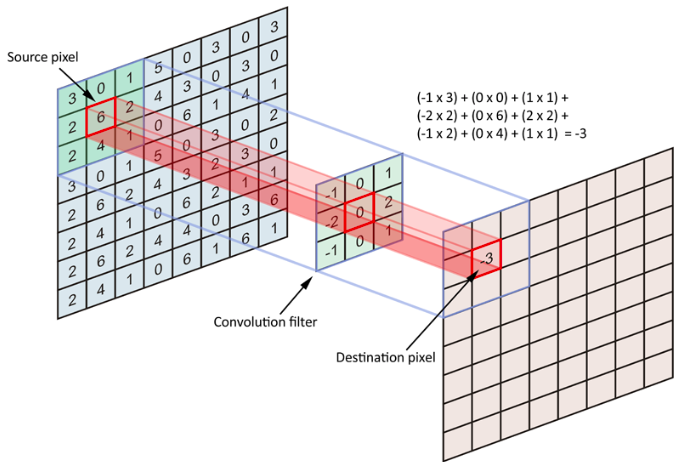
\includegraphics[width=\textwidth]{images/2d-Conv.png}
    \caption{Example of a single 3x3 convolution operation. The source image is convolved with a 3x3 kernel. The kernel's weights are determined using backpropagation. [cite source]}
    \label{fig:code:2DConv}
\end{figure}



\label{sec:code:inceptnet}
The inceptnet architecture [cite https://arxiv.org/abs/1409.4842] has been demonstrated by Böckenhoff [insert ref to Daniel's paper] to be effective on a simplified version of this problem.
In initial tests it was was very promising for this application and met an important boundary conditions, mainly the network fit into the available video memory on the system used to train the network.
Incept net uses a series of sub-networks, known as inception modules (see Fig \ref{fig:code:inceptmodule}).
Each inception module is made up of 3 convolutional paths (1x1, 3x3, and 5x5) and a pooling path.
To assure the outputs from each path have the same resolution, padding is added to the 3x3 and 5x5 convolutions.
The number of each convolutional filter can be adjusted at each step and the outputs are concatenated together.
The idea behind having multiple convolution sizes is that some features of the input might be lost if only size of kernel is applied.

\begin{figure}[htb]
    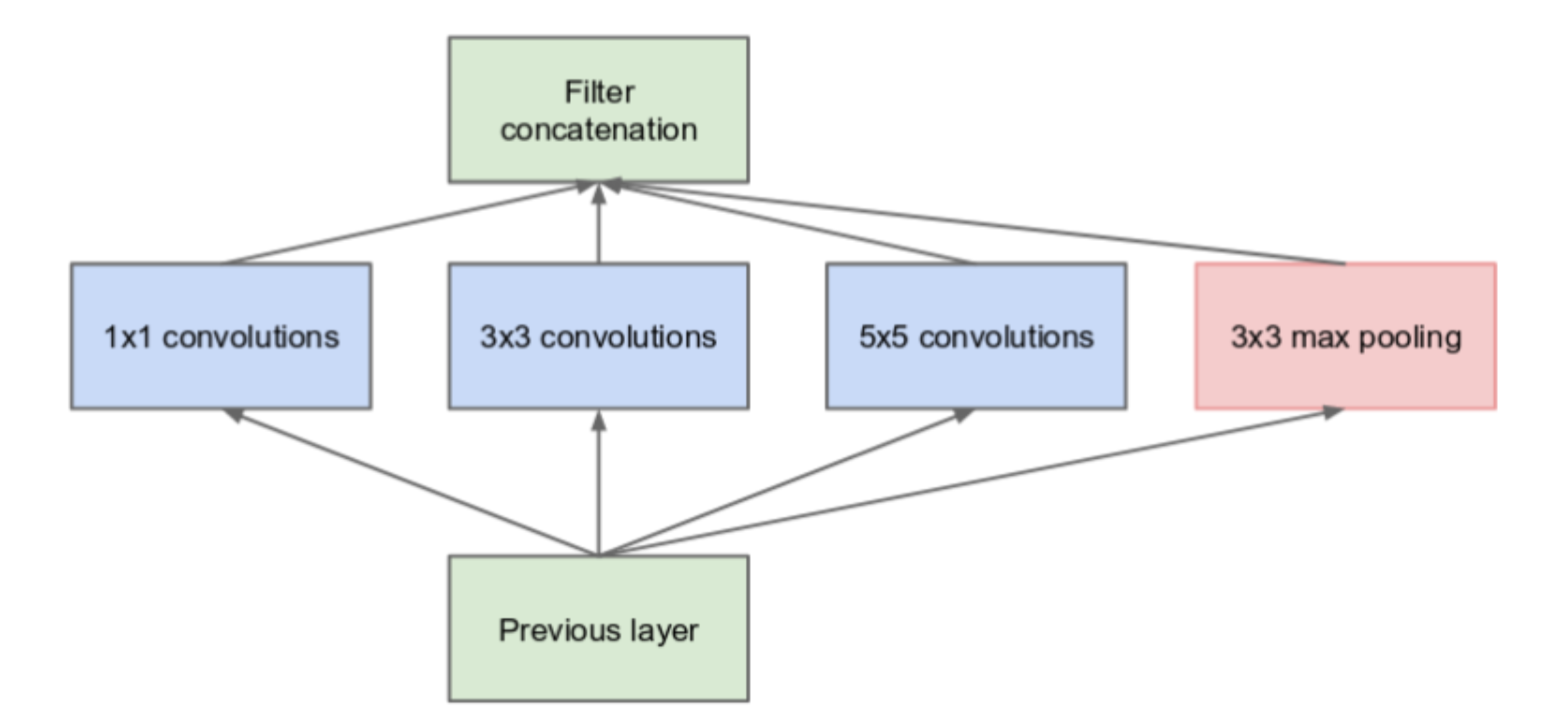
\includegraphics[width=\textwidth]{images/incept-simple.png}
    \caption{A diagram of the inception module. The inputs from the prior layer are fed into 4 paths, applying 1x1, 3x3, 5x5, convolutions with the final layer being 3x3 max pooling. The outputs of each layer are concatenated and passed to the next incept module. The number of 1x1, 3x3, and 5x5 convolutions per incept module can be adjusted.}
    \label{fig:code:inceptmodule}
\end{figure}

Incept modules also have two major advantages over classic deep convolutional networks, they require far fewer parameters and achieve better performance than their classic convolutional counterparts.
For example, using a 5x5 convolution to produce the same number of output channels as a incept module requires over 7 times the numbers of parameters and over 7 times the number of floating point operations.
This means that



Initially, the labels for the data set were not produce, since the simulations necessary to produce them take a great deal of time, simplified versions of the labels which just took into account the ratio of the ratio of the [Check with Andrea].
We can see in Eq. [Insert ref to Iota eq] that the first order term is the magnetic field produce by the coils so this will act as a good approximation.
The inceptnet architecture had three promising advantages over the other options.
The model size was small enough to fit entirely in the v-Ram of the available GPUs, the initial testing of the ResNet showing good success with the proxy for iota with limited tuning of the network, and the prior success with the architecture by Böckenhoff.
Because of these reasons it was the network selected to be used.


\label{sec:code:philosophy}
The design philosophy of this project was important. The code was designed to be a complete package, to be easily used by fellow colleges, and to work with the state of the art tools available in the machine learning space.
I went with the PyTorch framework, as many of my colleges used this as well, and the PyTorch Lightning package provided a powerful way to design an object-oriented package.
For lower-level operations, like managing and recording the network configuration files, hyperparmeter searches, as well as structuring and analyzing results, the package Hydra, developed by Facebook, was used.
Git was used for the version control system and DVC for data version control.
This project was profiled and optimized with help from the PyTorch Lightning profiler.
Code comments and documentation have been developed to help with quick adoption of the code for future use.
Since future changes to the divertor surface will result in drastically different inputs to the network, the code was designed to automatically scale with the inputs.
The design philosophy was focused on making a project that could be quickly and easily taken over by a future student and be powerful and flexible enough to work with expected changes in the future.



\label{sec:code:hyperparameters}

Once the broad architecture was selected the next step is to tune the model.
Tuning the model helps model level parameters, like the number of filters at a given module, to be optimized for the use case.
Tuning was done systematically with Optuna and results were recorded and compared using Tensorboard and MLFlow.
You can see from the table [Insert graph] the results of tuning the hyperparameter for the optimization step size $\alpha$.




% \section{Postcards: My Address}
% \label{sec:intro:address}

% \textbf{Ricardo Langner} \\
% Alfred-Schrapel-Str. 7 \\
% 01307 Dresden \\
% Germany



% \section{Motivation and Problem Statement}
% \label{sec:intro:motivation}

% \Blindtext[3][1] \cite{Jurgens:2000,Jurgens:1995,Miede:2011,Kohm:2011,Apple:keynote:2010,Apple:numbers:2010,Apple:pages:2010}

% \section{Results}
% \label{sec:intro:results}

% \Blindtext[1][2]

% \subsection{Some References}
% \label{sec:intro:results:refs}

% \cite{WEB:GNU:GPL:2010,WEB:Miede:2011}
% \Blindtext[1][1]

% \subsubsection{Methodology}
% \label{sec:intro:results:refs:method}

% \Blindtext[1][2]

% \paragraph{Strategy 1}
% \Blindtext[1][1]

% \begin{lstlisting}[language=Python, caption={This simple helloworld.py file prints Hello World.}\label{lst:pyhelloworld}]
% #!/usr/bin/env python
% print "Hello World"
% \end{lstlisting}

% \paragraph{Strategy 2}
% \Blindtext[1][1]

% \begin{lstlisting}[language=Python, caption={This is a bubble sort function.}\label{lst:pybubblesort}]
% #!/usr/bin/env python
% def bubble_sort(list):
%     for num in range(len(list)-1,0,-1):
%         for i in range(num):
%             if list[i]>list[i+1]:
%                 tmp = list[i]
%                 list[i] = list[i+1]
%                 list[i+1] = tmp

% alist = [34,67,2,4,65,16,17,95,20,31]
% bubble_sort(list)
% print(list)
% \end{lstlisting}

% \section{Thesis Structure}
% \label{sec:intro:structure}

% \textbf{Chapter \ref{sec:related}} \\[0.2em]
% \blindtext

% \textbf{Chapter \ref{sec:system}} \\[0.2em]
% \blindtext

% \textbf{Chapter \ref{sec:concepts}} \\[0.2em]
% \blindtext

% \textbf{Chapter \ref{sec:concepts}} \\[0.2em]
% \blindtext

% \textbf{Chapter \ref{sec:conclusion}} \\[0.2em]
% \blindtext
